%=======================02-713 LaTeX template, following the 15-210 template==================
%
% You don't need to use LaTeX or this template, but you must turn your homework in as
% a typeset PDF somehow.
%
% How to use:
%    1. Update your information in section "A" below
%    2. Write your answers in section "B" below. Precede answers for all 
%       parts of a question with the command "\question{n}{desc}" where n is
%       the question number and "desc" is a short, one-line description of 
%       the problem. There is no need to restate the problem.
%    3. If a question has multiple parts, precede the answer to part x with the
%       command "\part{x}".
%    4. If a problem asks you to design an algorithm, use the commands
%       \algorithm, \correctness, \runtime to precede your discussion of the 
%       description of the algorithm, its correctness, and its running time, respectively.
%    5. You can include graphics by using the command \includegraphics{FILENAME}
%
\documentclass[11pt]{article}
\usepackage{amsmath,amssymb,amsthm}
\usepackage{graphicx}
\usepackage[margin=1in]{geometry}
\usepackage{fancyhdr}
\usepackage{tabularx}
	\newcolumntype{L}{>{\raggedright\arraybackslash}X}
\usepackage{adjustbox}
\usepackage{xspace}
\setlength{\parindent}{0pt}
\setlength{\parskip}{5pt plus 1pt}
\setlength{\headheight}{13.6pt}
\newcommand\question[2]{\vspace{.25in}\hrule\textbf{#1: #2}\vspace{.5em}\hrule\vspace{.10in}}
\renewcommand\part[1]{\vspace{.10in}\textbf{(#1)}\par}
\newcommand\algorithm{\vspace{.10in}\textbf{Algorithm: }}
\newcommand\correctness{\vspace{.10in}\textbf{Correctness: }}
\newcommand\runtime{\vspace{.10in}\textbf{Running time: }}
\pagestyle{fancyplain}
\lhead{\textbf{\NAME}}
\chead{\textbf{{\COURSE} HW\HWNUM}}
\rhead{\today}
\begin{document}\raggedright
%Section A==============Change the values below to match your information==================
\newcommand\NAME{Eric Altenburg}  % your name
\newcommand\COURSE{CS-383}
\newcommand\HWNUM{4}              % the homework number
%Section B==============Put your answers to the questions below here=======================

% no need to restate the problem --- the graders know which problem is which,
% but replacing "The First Problem" with a short phrase will help you remember
% which problem this is when you read over your homeworks to study.

\begin{center}
	\textit{\textbf{Pledge:} I pledge my honor that I have abided by the Stevens Honor System.} - \textbf{\NAME}
\end{center}


\question{5.1}{Page 497} % All same

	\part{5.1.1}
		\textbf{2}\par
	
	\part{5.1.2}
		\textbf{I, J, B[I][0]}\par
	
	\part{5.1.3}
		\textbf{A[I][J]}\par
	

\question{5.2}{Page 498} % Same all
	
	\part{5.2.1}
		\begin{center}
			\begin{tabular}{|c|c|c|c|c|}
				\hline
				Word Address & Binary Address & Tag & Index & Hit/Miss\\
				\hline
				0x03 & 0000 0011 & 0 & 3 & M\\
				\hline
				0xb4 & 1011 0100 & b & 4 & M\\
				\hline
				0x2b & 0010 1011 & 2 & b & M\\
				\hline
				0x02 & 0000 0010 & 0 & 2 & M\\
				\hline
				0xbf & 1011 1111 & b & f & M\\
				\hline
				0x58 & 0101 1000 & 5 & 8 & M\\
				\hline
				0xbe & 1011 1110 & b & e & M\\
				\hline
				0x0e & 0000 1110 & 0 & e & M\\
				\hline
				0xb5 & 1011 0101 & b & 5 & M\\
				\hline
				0x2c & 0010 1100 & 2 & c & M\\
				\hline
				0xba & 1011 1010 & b & a & M\\
				\hline
				0xfd & 1111 1101 & f & d & M\\
				\hline
			\end{tabular}
		\end{center}
	
	\newpage
	\part{5.2.2}
		\begin{center}
			\begin{tabular}{|c|c|c|c|c|c|}
				\hline
				Word Address & Binary Address & Tag & Index & Offset & Hit/Miss\\
				\hline
				0x03 & 0000 0011 & 0 & 1 & 1 & M\\
				\hline
				0xb4 & 1011 0100 & b & 2 & 0 & M\\
				\hline
				0x2b & 0010 1011 & 2 & 5 & 1 & M\\
				\hline
				0x02 & 0000 0010 & 0 & 1 & 0 & H\\
				\hline
				0xbf & 1011 1111 & b & 7 & 1 & M\\
				\hline
				0x58 & 0101 1000 & 5 & 4 & 0 & M\\
				\hline
				0xbe & 1011 1110 & b & 6 & 0 & H\\
				\hline
				0x0e & 0000 1110 & 0 & 7 & 0 & M\\
				\hline
				0xb5 & 1011 0101 & b & 2 & 1 & H\\
				\hline
				0x2c & 0010 1100 & 2 & 6 & 0 & M\\ 
				\hline
				0xba & 1011 1010 & b & 5 & 0 & M\\
				\hline
				0xfd & 1111 1101 & f & 6 & 1 & M\\
				\hline
			\end{tabular}
		\end{center}
	
	\part{5.2.3}
	Just wanted to preface this by saying that if there are any discrepancies between the Word Address, Binary Address, and Tag across the tables, then it is simply a mistake. All three tables should have the same numbers/values for the aforementioned columns.\par
		\begin{center}
		\begin{tabular}{|c|c|c|c|c|c|c|c|c|}
			\hline
			\multicolumn{5}{|c|}{\text{Cache 1}}\\
			\hline
			Word Address & Binary Address & Tag & Index & Hit/Miss\\
			\hline
			0x03 & 0000 0011 & 0x00 & 3 & M\\
			\hline
			0xb4 & 1011 0100 & 0x16 & 4 & M\\
			\hline
			0x2b & 0010 1011 & 0x05 & 3 & M\\
			\hline
			0x02 & 0000 0010 & 0x00 & 2 & M\\
			\hline
			0xbf & 1011 1111 & 0x17 & 7 & M\\
			\hline
			0x58 & 0101 1000 & 0x0b & 0 & M\\
			\hline
			0xbe & 1011 1110 & 0x17 & 6 & M\\
			\hline
			0x0e & 0000 1110 & 0x01 & 6 & M\\
			\hline
			0xb5 & 1011 0101 & 0x16 & 5 & M\\
			\hline
			0x2c & 0010 1100 & 0x05 & 4 & M\\
			\hline
			0xba & 1011 1010 & 0x17 & 2 & M\\
			\hline
			0xfd & 1111 1101 & 0x1f & 5 & M\\
			\hline
		\end{tabular}
		\end{center}\par
		Cache 1 Miss Rate = \textbf{100\%}\par
		Cache 1 Total Cycles  = \textbf{324}\par
		\begin{center}
		\begin{tabular}{|c|c|c|c|c|c|c|c|c|}
			\hline
			\multicolumn{5}{|c|}{\text{Cache 2}}\\
			\hline
			Word Address & Binary Address & Tag & Index & Hit/Miss\\
			\hline
			0x03 & 0000 0011 & 0x00 & 1 & M\\
			\hline
			0xb4 & 1011 0100 & 0x16 & 2 & M\\
			\hline
			0x2b & 0010 1011 & 0x05 & 1 & M\\
			\hline
			0x02 & 0000 0010 & 0x00 & 1 & M\\
			\hline
			0xbf & 1011 1111 & 0x17 & 3 & M\\
			\hline
			0x58 & 0101 1000 & 0x0b & 0 & M\\
			\hline
			0xbe & 1011 1110 & 0x17 & 3 & H\\
			\hline
			0x0e & 0000 1110 & 0x01 & 3 & M\\
			\hline
			0xb5 & 1011 0101 & 0x16 & 2 & H\\
			\hline
			0x2c & 0010 1100 & 0x05 & 2 & M\\
			\hline
			0xba & 1011 1010 & 0x17 & 1 & M\\
			\hline
			0xfd & 1111 1101 & 0x1f & 2 & M\\
			\hline
		\end{tabular}
		\end{center}\par
    		Cache 2 Miss Rate = \textbf{83\%}\par
		Cache 2 Total Cycles = \textbf{286}\par
		This is the cache that has the best performance.\par
		\begin{center}
		\begin{tabular}{|c|c|c|c|c|c|c|c|c|}
			\hline
			\multicolumn{5}{|c|}{\text{Cache 3}}\\
			\hline
			Word Address & Binary Address & Tag & Index & Hit/Miss\\
			\hline
			0x03 & 0000 0011 & 0x00 & 0 & M\\
			\hline
			0xb4 & 1011 0100 & 0x16 & 1 & M\\
			\hline
			0x2b & 0010 1011 & 0x05 & 0 & M\\
			\hline
			0x02 & 0000 0010 & 0x00 & 0 & M\\
			\hline
			0xbf & 1011 1111 & 0x17 & 1 & M\\
			\hline
			0x58 & 0101 1000 & 0x0b & 0 & M\\
			\hline
			0xbe & 1011 1110 & 0x17 & 1 & H\\
			\hline
			0x0e & 0000 1110 & 0x01 & 1 & M\\
			\hline
			0xb5 & 1011 0101 & 0x16 & 1 & M\\
			\hline
			0x2c & 0010 1100 & 0x05 & 1 & M\\
			\hline
			0xba & 1011 1010 & 0x17 & 0 & M\\
			\hline
			0xfd & 1111 1101 & 0x1F & 1 & M\\
			\hline
		\end{tabular}
		\end{center}\par
		Cache 3 Miss Rate = \textbf{92\%}\par
		Cache 3 Total Cycles = \textbf{335}\par
		As mentioned above, cache 2 has the best performance.\par
		
		
\question{5.5}{Page 499} % Same all

	\part{5.5.1}
		All of the cache blocks have 4 8-byte words (assuming each word is 8-bytes, but if they were to be 4-bytes per word, then there would be 8 4-byte words).\par
		Offset total =  5 bits with 3 of the 5 being the word offset and the last 2 being for the block offset.\par
		The 2 bits enumerate $2^{2}=4$ words.\par
	
	\part{5.5.2}
		With 5 index bits, you can have $2^{5} = 32$ lines in the cache.\par
	
	\part{5.5.3}
		$32 * 4 * 8 = 8192$ bits.\par
		$8192 + (54*32) + (1 * 32)=9952$ bits.\par
		$\frac{9952}{8192}=\textbf{1.21}$\par
	
	\part{5.5.4}
		\begin{center}
			\begin{tabular}{|c|c|c|c|c|c|c|}
				\hline
				Byte Address & Binary Address & Tag & Index & Offset & Hit/Miss & Bytes Replaced\\
				\hline
				0x00 & 0000 0000 0000 & 0x0 & 0x00 & 0x00 & M &\\
				\hline
				0x04 & 0000 0000 0100 & 0x0 & 0x00 & 0x04 & H &\\
				\hline
				0x10 & 0000 0001 0000 & 0x0 & 0x00 & 0x10 & H &\\
				\hline
				0x84 & 0000 1000 0100 & 0x0 & 0x04 & 0x04 & M &\\
				\hline
				0xe8 & 0000 1110 1000 & 0x0 & 0x07 & 0x08 & M &\\
				\hline
				0xa0 & 0000 1010 0000 & 0x0 & 0x05 & 0x00 & M&\\
				\hline
				0x400 & 0100 0000 0000 & 0x1 & 0x00 & 0x00 & M & 0x00-0x1F\\
				\hline
				0x1e & 0000 0001 1110 & 0x0 & 0x00 & 0x1e & M & 0x400-0x41F\\
				\hline
				0x8c & 0000 1000 1100 & 0x0 & 0x04 & 0x0c & H &\\
				\hline
				0xc1c & 1100 0001 1100 & 0x3 & 0x00 & 0x1c & M & 0x00-0x1F\\
				\hline
				0xb4 & 0000 1011 0100 & 0x0 & 0x05 & 0x14 & H &\\
				\hline
				0x884 & 1000 1000 0100 & 0x2 & 0x04 & 0x04 & M & 0x80-0x9f\\
				\hline
			\end{tabular}
		\end{center}\par
	
	\part{5.5.5}
		$\frac{4}{12}=\textbf{33\%}$\par
	
	\part{5.5.6}
		\begin{tabular}{*3c}
			$<$0, & 3, & Mem[0xC00] - Mem[0xC1F]$>$\\
			$<$4, & 2, & Mem[0x880] - Mem[0x89f]$>$\\
			$<$5, & 0, & Mem[0x0A0] - Mem[0x0Bf]$>$\\
			$<$7, & 0, & Mem[0x0e0] - Mem[0x0ff]$>$\\
		\end{tabular}\par
	

\question{5.9}{Page 501} % Same all
	
	\part{5.9.1}
		AMAT for B = 8: $0.040 * (20 * 8) = \textbf{6.4}$\par
		AMAT for B = 16: $0.030 * (20 * 16) = \textbf{9.6}$\par
		AMAT for B = 32: $0.020 * (20 * 32) = \textbf{12.8}$\par
		AMAT for B = 64: $0.015 * (20 * 64) = \textbf{19.2}$\par
		AMAT for B = 128: $0.010 * (20 * 128) = \textbf{25.6}$\par
		A block size of B = 8 is optimal.\par
		
	\part{5.9.2}
		AMAT for B = 8: $0.040 * (24 + 8) = \textbf{1.28}$\par
		AMAT for B = 16: $0.030 * (24 + 16) = \textbf{1.20}$\par
		AMAT for B = 32: $0.020 * (24 + 32) = \textbf{1.12}$\par
		AMAT for B = 64: $0.015 * (24 + 64) = \textbf{1.32}$\par
		AMAT for B = 128: $0.010 * (24 + 128) = \textbf{1.52}$\par
		A block size of B = 32 is optimal.\par
		
	\part{5.9.3}
		A block size of B = 128 is optimal because when you minimize the miss rate, the total miss latency is also reduced.\par
		

\question{5.11}{Page 502} % Same all

	\part{5.11.1}
		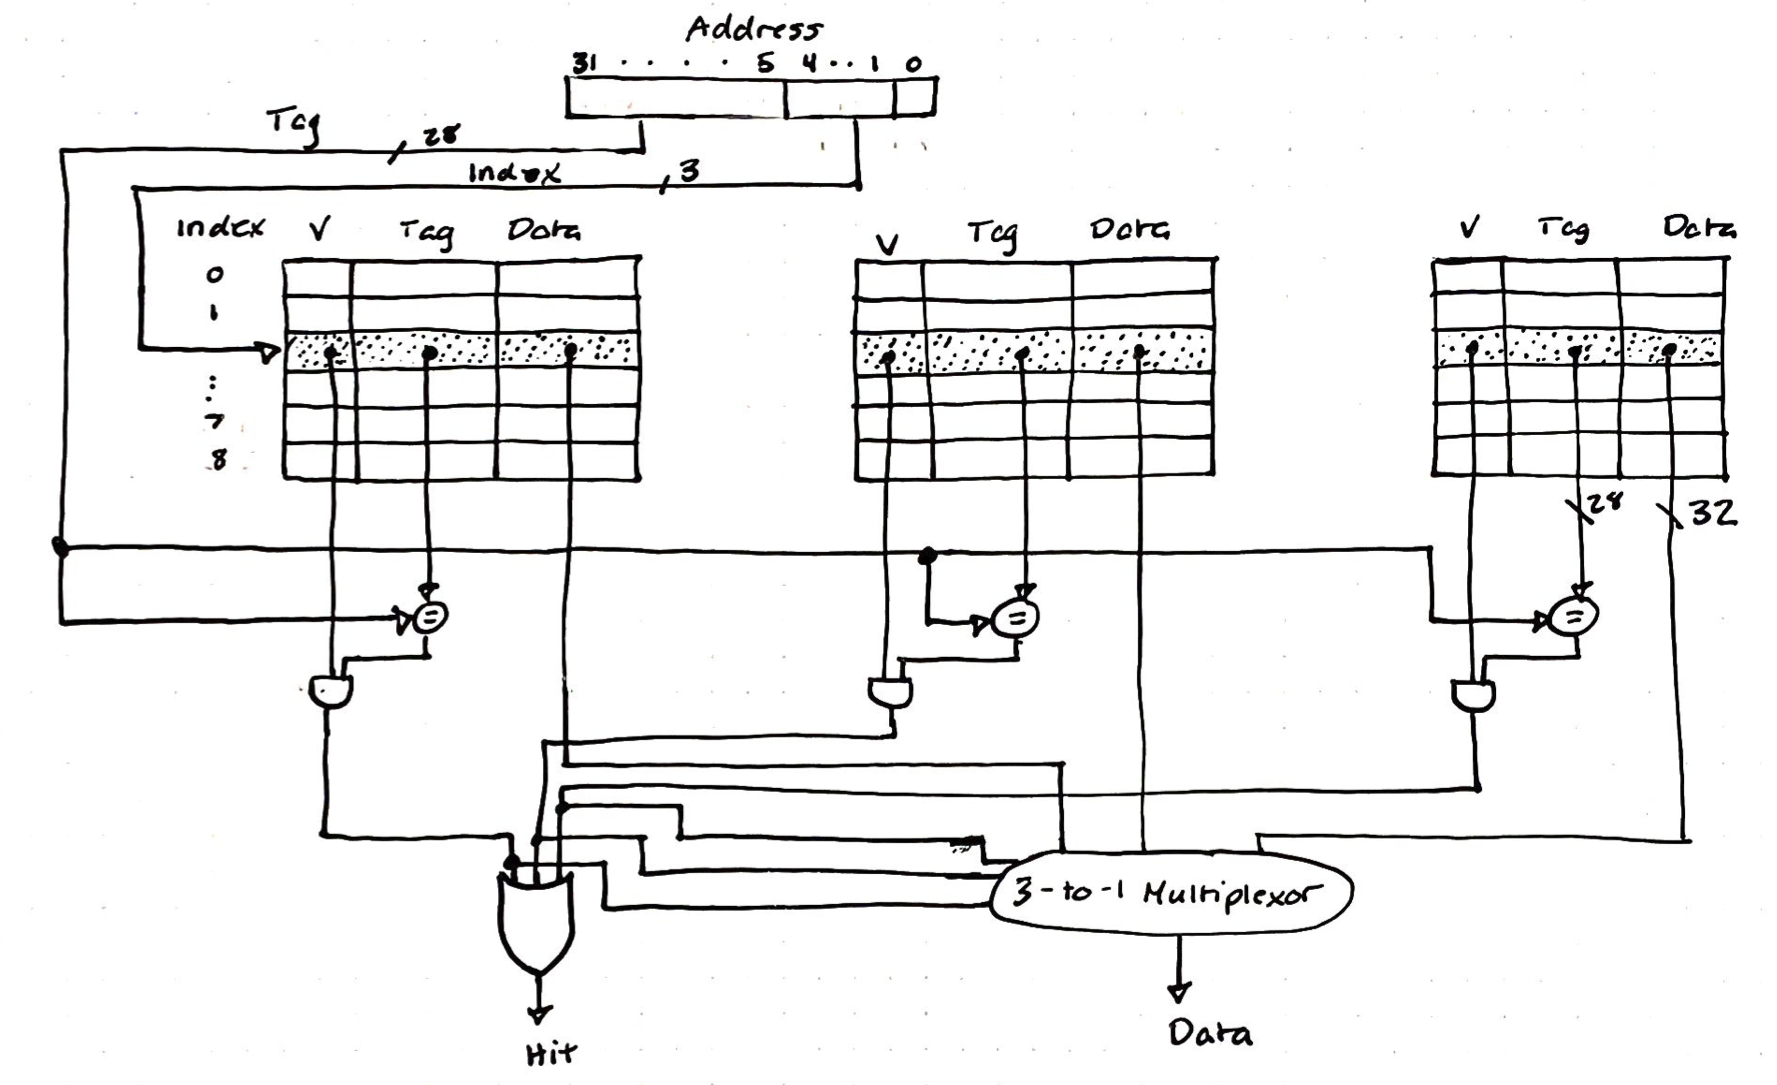
\includegraphics{images/yeet.png}\par
		Since each block can hold 2 words, the word offset bits = $log_{2}2$ = 1 bit\par
		Number of cache slots = $\frac{cache\:size}{block\:size} = \frac{48}{2}$ = 24 slots\par
		Number of sets = $\frac{24}{3}$ = 8\par
		Set Offset Bits = $log_{2}8$ = 3 bits\par
		$32-3-1$= 28 bits for the tag \par
	
	\newpage
	\part{5.11.2}
		\begin{center}
		\begin{adjustbox}{width=!, height=11cm}
			\begin{tabularx}{\linewidth}{|L|L|c|c|c|c|L|L|c|}
				\hline
				Word Address & Binary Address & Tag & Index & Offset & Hit/Miss & Way 0 & Way 1 & Way 2\\
				\hline
				0x03 & 0000 0011 & 0x0 & 1 & 1 & M & T(1)=0 & &\\
				\hline
				0xb4 & 1011 0100 & 0xb & 2 & 0 & M & T(1)=0 T(2)=b & &\\
				\hline
				0x2b & 0010 1011 & 0x2 & 5 & 1 & M & T(1)=0 T(2)=b T(5)=2 &&\\
				\hline
				0x02 & 0000 0010 & 0x0 & 1 & 0 & H & T(1)=0 T(2)=b T(5)=2 &&\\
				\hline
				0xbe & 1011 1110 & 0xb & 7 & 0 & M & T(1)=0 T(2)=b T(5)=2 T(7)=b &&\\
				\hline
				0x58 & 0101 1000 & 0x5 & 4 & 0 & M & T(1)=0 T(2)=b T(5)=2 T(7)=b T(4)=5 &&\\
				\hline
				0xbf & 1011 1111 & 0xb & 7 & 1 & H & T(1)=0 T(2)=b T(5)=2 T(7)=b T(4)=5  &&\\
				\hline
				0x0e & 0000 1110 & 0x0 & 7 & 0 & M & T(1)=0 T(2)=b T(5)=2 T(7)=b T(4)=5 & T(7)=0 &\\
				\hline
				0x1f & 0001 1111 & 0x1 & 7 & 1 & M & T(1)=0 T(2)=b T(5)=2 T(7)=b T(4)=5  & T(7)=0 & T(7)=1\\
				\hline
				0xb5 & 1011 0101 & 0xb & 2 & 1 & H & T(1)=0 T(2)=b T(5)=2 T(7)=b T(4)=5 & T(7)=0 & T(7)=1\\
				\hline
				0xbf & 1011 1111 & 0xb & 7 & 1 & H & T(1)=0 T(2)=b T(5)=2 T(7)=b T(4)=5 & T(7)=0 & T(7)=1\\
				\hline
				0xba & 1011 1010 & 0xb & 5 & 0 & M & T(1)=0 T(2)=b T(5)=2 T(7)=b T(4)=5 & T(7)=2 T(5)=b & T(7)=1\\
				\hline
				0x2e & 0010 1110 & 0x2 & 7 & 0 & M & T(1)=0 T(2)=b T(5)=2 T(7)=b T(4)=5 & T(7)=2 T(5)=b & T(7)=1\\
				\hline
				0xce & 1100 1110 & 0xc & 7 & 0 & M & T(1)=0 T(2)=b T(5)=2 T(7)=b T(4)=5  & T(7)=2 T(5)=b & T(7)=c\\
				\hline
			\end{tabularx}
		\end{adjustbox}
		\end{center}	
	\newpage
	
	\part{5.11.3}
		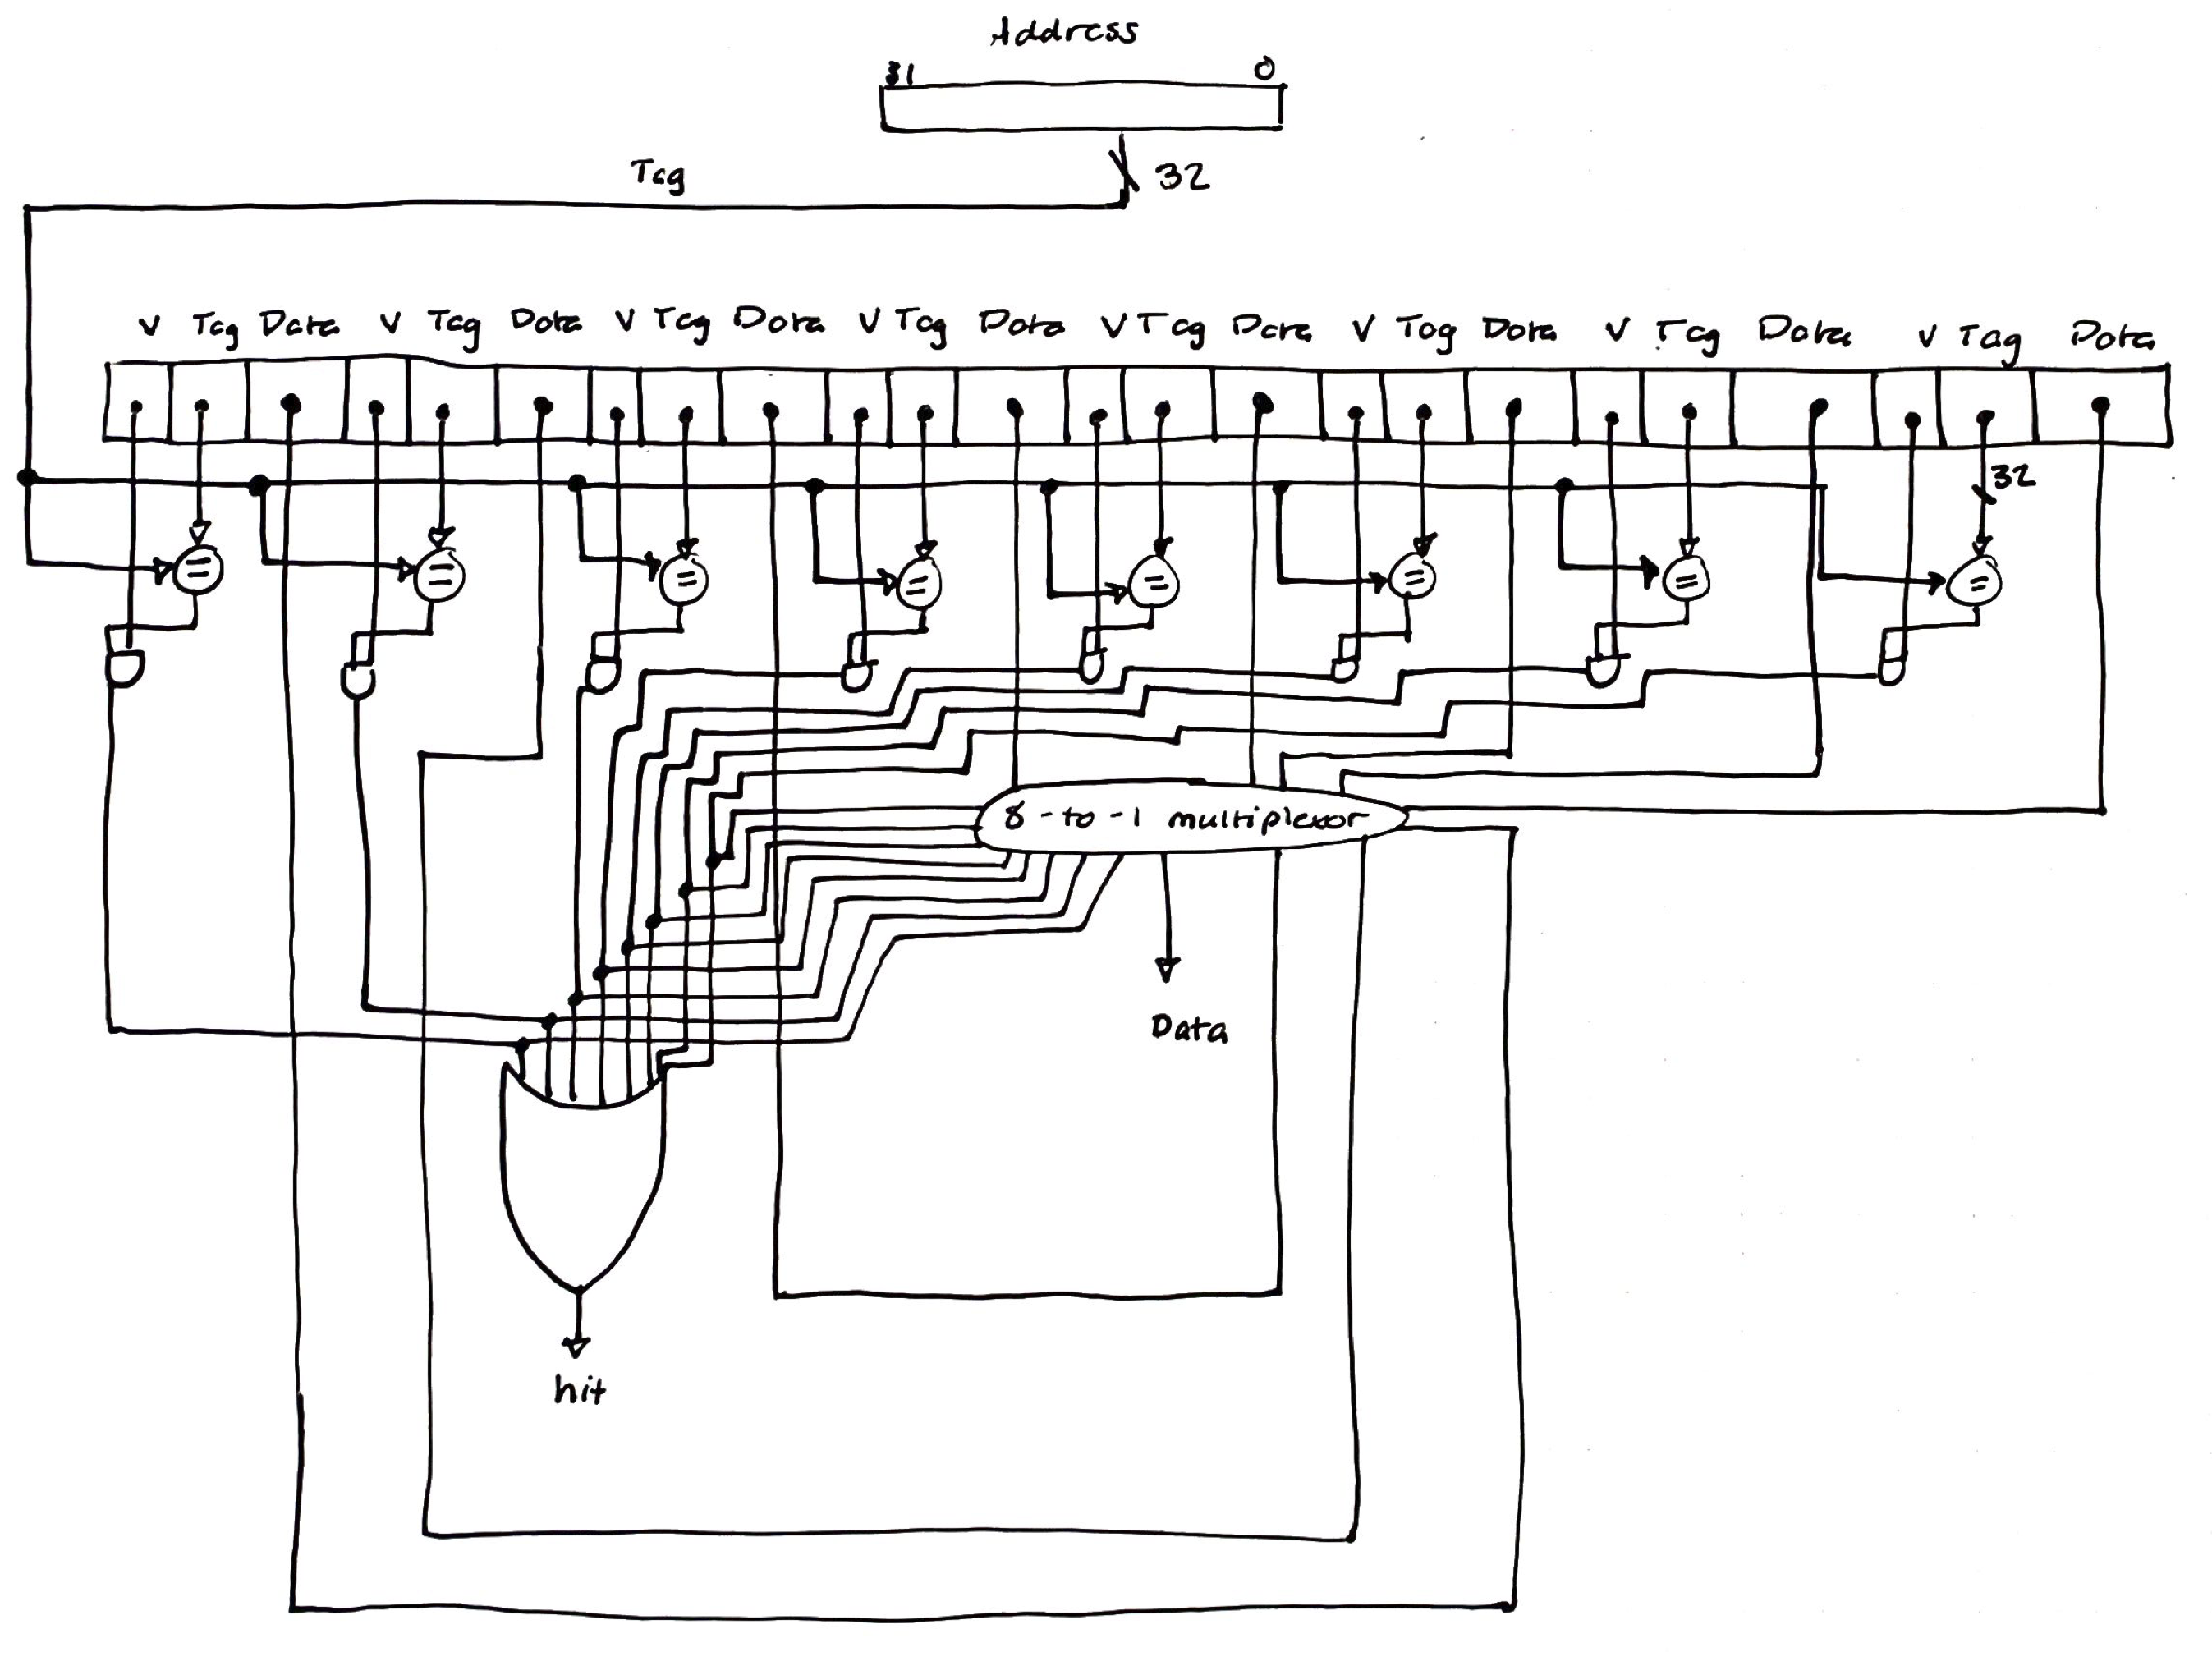
\includegraphics[width=\textwidth]{images/yeet(2).png}\par
		Since each block can hold 1 word, the word offset bits = $log_{2}1$ = 0 bits\par
		Number of cache slots = $\frac{cache\:size}{block\:size} = \frac{8}{1}$ = 8 slots\par
		$32-0$= 32 bits for the tag \par


\question{5.13}{Page 504} % Same all

	\part{5.13.1}
		For a MTTF of 3 years and a MTTR of 1 day, the MTBF is \textbf{1096 days or 26304 hours}.\par
	
	\part{5.13.2}
		$\frac{1095}{1096}=\textbf{99.90875\%}.$\par
	
	\part{5.13.3}
		As the MTTR approaches 0, the \textbf{availability will approach 1}. Since drives are becoming more and more inexpensive, the possibility of having a MTTR of 0 for hardware is becoming more likely, but replacing the data would be very time consuming and this is often overlooked.\par
	
	\part{5.13.4}
		\textbf{Availability would be a high number if MTTR were to vastly increase} as it plays a significant role in calculations, but if MTTF were to grow considerably, then the availability would be high as well. It all depends on the ratio of the values of MTTR to MTTF as if MTTF is a large number in comparison to MTTR, MTTR's values will not be meaningful.\par


\end{document}